\documentclass{cubeamer}

\title{Performance-Portable Implicit Scale-Resolving Compressible Flow Using libCEED}
\subtitle{SIAM CSE 2023}
\author[James Wright]{James Wright, Jed Brown, Kenneth Jansen, Leila Ghaffari}
\date{February 27, 2023} % or whatever the date you are presenting in is
\institute[University of Colorado Boulder]{Ann and H.J. Smead Department of Aerospace Engineering Sciences}

\usefonttheme{professionalfonts} % required for mathspec
\usepackage{mathspec}
\setmathsfont{Latin Modern Math}

\usepackage{todonotes}
\presetkeys{todonotes}{inline}{}

\usepackage{esdiff}
\usepackage[scr=boondoxo]{mathalpha} % Get better script L
\usepackage{minted}

\newminted{c}{fontsize=\tiny,
            linenos,
            numbersep=2pt,
            gobble=0,
            frame=lines,
            bgcolor=bg,
            framesep=3mm}

\renewcommand{\vec}[1]{\bm{#1}}
\newcommand{\defeq}{\vcentcolon=}
\newcommand{\eqdef}{=\vcentcolon}
\DeclarePairedDelimiter{\angbr}{\langle}{\rangle}
\DeclareMathOperator{\Span}{span}
\newcommand{\avg}[1]{\angbr{#1}}

\newcommand<>{\uncoverubrace}[2]{%
  \onslide#3 \underbrace{ \onslide<1->%
  #1%
  \onslide#3 }_{#2} \onslide<1->%
}
\newcommand<>{\uncoverobrace}[2]{%
  \onslide#3 \overbrace{ \onslide<1->%
  #1%
  \onslide#3 }^{#2} \onslide<1->%
}

\usepackage{xcolor}
\newcommand{\Part}{\textcolor[HTML]{ad0000}{\mathcal{P}}}
\newcommand{\PartT}{\textcolor[HTML]{ad0000}{\mathcal{P}^T}}
\newcommand{\Elem}{\mathcal{E}}
\newcommand{\ElemT}{\mathcal{E}^T}
\newcommand{\Bas}{\textcolor[HTML]{0f75ff}{B}}
\newcommand{\BasT}{\textcolor[HTML]{0f75ff}{B^T}}
\newcommand{\DQfunc}{\textcolor[HTML]{009900}{D}}
\newcommand{\Qfunc}[1]{\textcolor[HTML]{009900}{#1}}
\newcommand{\nelm}{{n_{\mathrm{elm}}}}
\newcommand{\ndof}{{n_{\mathrm{dof}}}}
\newcommand{\nquad}{{n_{\mathrm{quad}}}}
\newcommand{\derd}{{{\mathrm{d}}}}

% Colors for tikz and mat-mult solids chart
\definecolor{solids_yellow}{HTML}{E0BD6C}
\definecolor{solids_red}{HTML}{C98190}
\definecolor{solids_blue}{HTML}{4686C7}

\begin{document}

\maketitle

\cutoc

%% TODOs
% [ ] Add references and thanks to support
% [ ] Mention Solids performance in libCEED intro (gives better motivation)
% [-] (Possibly) remove references to recirculation from BC discussion (check with Ken and Jed)
% [-] Cleanup performance bar graph (get Q_1 results for same size problem, change label names)
% [-] Slide 5: Fix up the overlay order with the "Simplify into residual form"
% [-] Reverse legend order in bar chart

\section{libCEED Overview}

\begin{frame}{What is libCEED?}

    \begin{itemize}
        \item<+-> C library for element-based discretizations
            \begin{itemize}
                \item Bindings available for Fortran, Rust, Python, and Julia
            \end{itemize}
        \item<+-> Designed for matrix-free operator evaluation
        \item<+-> Portable to different hardware via computational backends
            \begin{itemize}
                \item Code that runs on CPU also runs on GPU without changes
                \item Computational backend selectable at runtime, using runtime compilation
            \end{itemize}
        \item<+-> Geared toward high-order finite element discretizations
        \item<+-> Performance demonstrated for solids in Brown \textit{et al.} 2022\footnote<.->{\textit{Performance Portable Solid Mechanics via Matrix-Free \(p\)-Multigrid}, Brown \textit{et al.}, arXiv:2204.01722}
            \begin{itemize}
                \item Want to apply those methods and lessons-learned to fluids
            \end{itemize}
    \end{itemize}

\end{frame}
%1:40

\begin{frame}{Finite Element Operator Decomposition}
    \onslide<2->{
        \begin{tikzpicture}

            % Include the image in a node
            \node [
            above right,
            inner sep=0] (image) at (0,0) {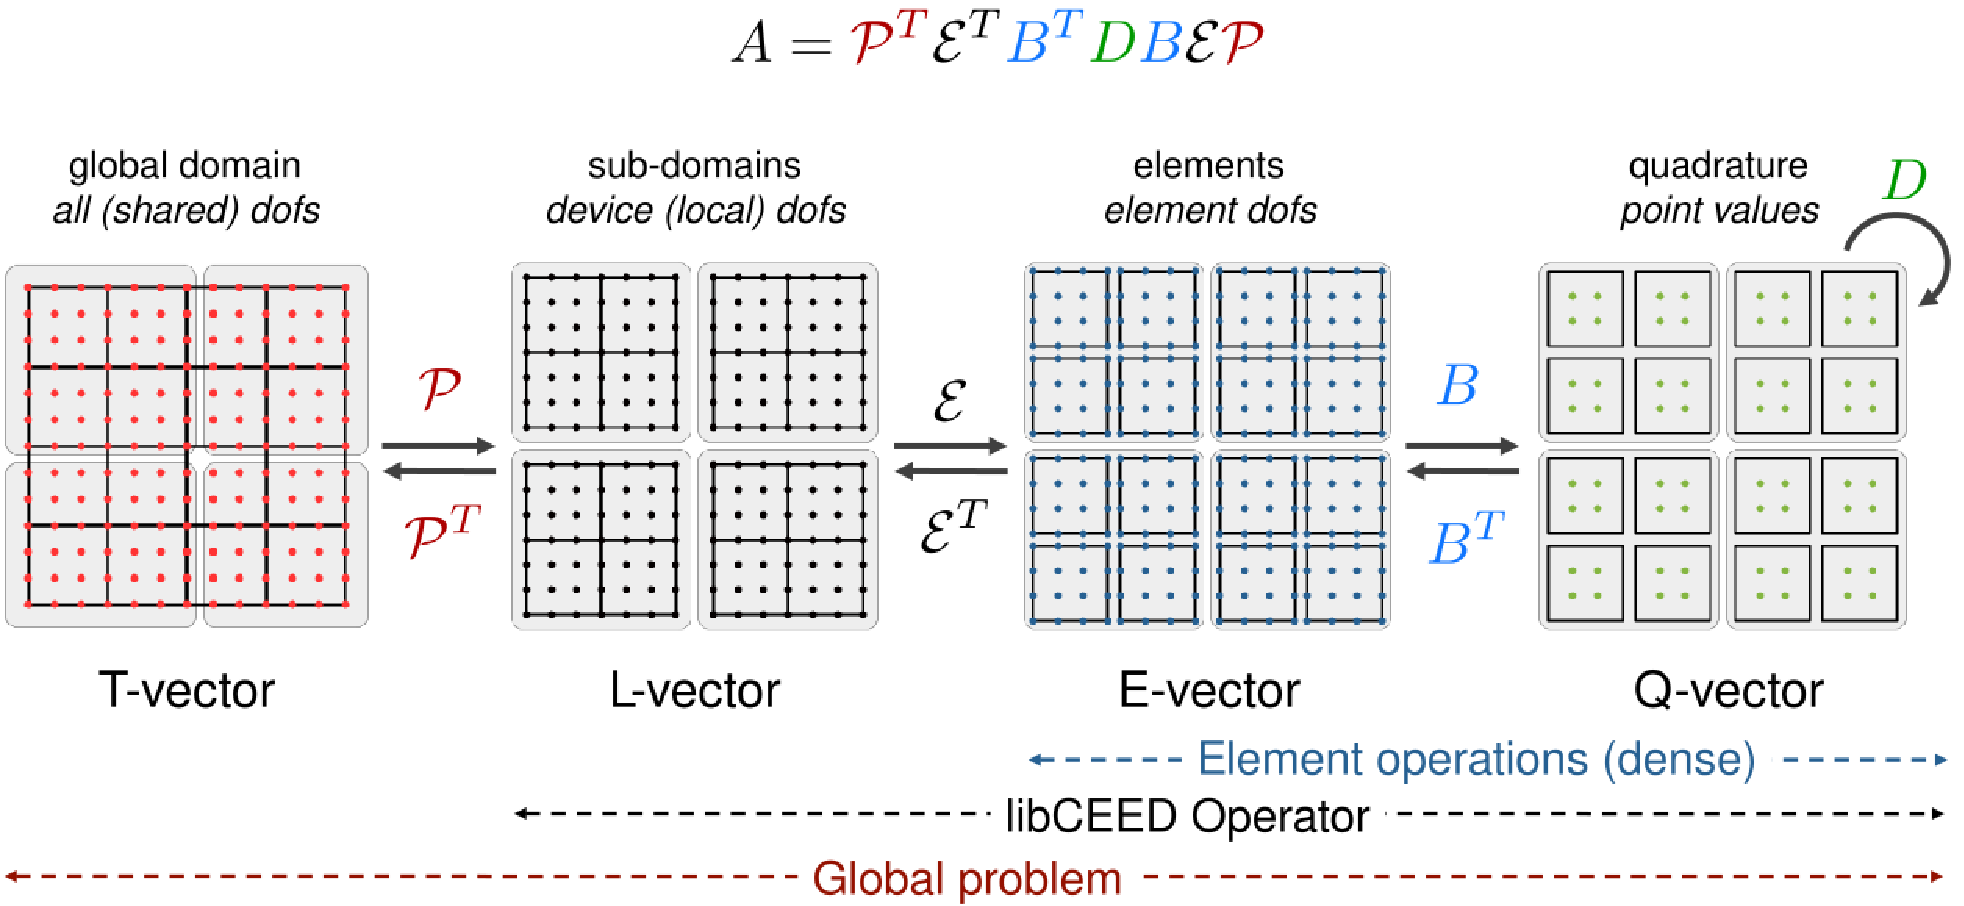
\includegraphics[width=0.9\textwidth]{img/FEMDecomp.pdf}};

            % Create scope with normalized axes
            \begin{scope}[
                x={($0.1*(image.south east)$)},
                y={($0.1*(image.north west)$)}]

                % % Grid
                %     \draw[lightgray,step=1] (image.south west) grid (image.north east);
                %
                % % Axes' labels
                %     \foreach \x in {0,1,...,10} { \node [below] at (\x,0) {\x}; }
                %     \foreach \y in {0,1,...,10} { \node [left] at (0,\y) {\y};}

                \invisible<3->{\draw[ultra thin,white,fill=white] (10, 0.6) rectangle (1.9, 9);}
                \invisible<4->{\draw[ultra thin,white,fill=white] (10, 1.4) rectangle (4.5, 9);}
                \invisible<5->{\draw[ultra thin,white,fill=white] (10, 1.4) rectangle (7.1, 9);}
                \invisible<6->{\draw[ultra thin,white,fill=white] (10, 7.7) rectangle (9.3, 9);}
                \invisible<7->{\draw[ultra thin,white,fill=white] (10, 0) rectangle (0, 2);}
            \end{scope}

            % TODO Add a "processors" tag to the image

        \end{tikzpicture}
    }

\end{frame}

\section{Compressible Fluid Equations in libCEED}

\begin{frame}{Compressible Navier-Stokes}


    \begin{equation*}
        \bm{A_0}\bm{Y}_{,t} + \bm{F}_{i,i}(\bm{Y}) - S(\bm{Y}) = 0
    \end{equation*}

    for

    \begin{equation*}
        \bm{A_0}
        \underbrace{\begin{bmatrix}
            p \\
            u_i\\
            T
    \end{bmatrix}}_{\bm{Y}} =
        \begin{bmatrix}
            \rho \\
            \rho u_i\\
            \rho e
        \end{bmatrix}, \quad
    \bm{F}_i(\bm{Y}) =
    \underbrace{
        \begin{pmatrix}
            \rho u_i\\
            \rho u_i u_j + p \delta_{ij} \\
            (\rho e + p)u_i
        \end{pmatrix}}_{\bm F_i^{\mathrm{adv}}} +
    \underbrace{
        \begin{pmatrix}
        0 \\
        -  \sigma_{ij} \\
        - \rho u_j  \sigma_{ij} - k T_{,i}
        \end{pmatrix}}_{\bm F_i^{\mathrm{diff}}}, \quad
    S(\bm{Y}) =
    - \begin{pmatrix}
        0\\
        \rho \bm{g} \\
        0
    \end{pmatrix}
    \end{equation*}
\end{frame}

\begin{frame}{Compressible Navier-Stokes for Continuous-Galerkin FEM}

    Find \(\bm{Y}\in \mathcal{S}^h \, , \; \forall \bm v \in \mathcal{V}^h\)
    \begin{equation*}
        \begin{aligned}
            \only<-+>{\quad\ \ \,}\int_{\Omega} \bm v \cdot \left[ \bm{A_0}\bm{Y}_{,t} - \bm{S}(\bm{Y}) \right]  \,\dif \Omega
            \only<-.>{
                + \int_{\Omega} \bm{v} \cdot \bm{F}_{i,i}(\bm{Y})\, \dif\Omega
            }
            \uncover<+->{
                - \int_{\Omega} \bm{v}_{,i} \cdot \bm{F}_i(\bm{Y})\, \dif\Omega
                + \int_{\partial \Omega} \bm v \cdot \bm{F}_i(\bm{Y}) \cdot \widehat{\bm{n}}_i \,\dif \partial \Omega & \\
            }
            \onslide<+->{\underbrace{+ \int_{\Omega} \mathscr{L}^{\mathrm{adv}}(\bm v)\bm{\tau} \, \left[\bm{A_0}\bm{Y}_{,t} + \bm{F}_{i,i}(\bm{Y}) - S(\bm{Y})
            \right] \,\dif \Omega}_{\textrm{SUPG}} &= 0}
        \end{aligned}
    \end{equation*}
    \vspace{-10pt}
    \onslide<+->{
        Simplify into residual form:
        \begin{align*}
            \mathcal{G}(\bm{Y}_{,t}, \bm{Y}) &=0 \\
            \onslide<+->{\Rightarrow \quad \PartT \ElemT \BasT \Qfunc{G} \Bas \Elem \Part
                \begin{bmatrix}
                    \bm{Y}_{,t} \\
                    \bm{Y}
                \end{bmatrix} &= 0}
        \end{align*}
    }
\end{frame}

\section{Efficient Implicit Timestepping}

\begin{frame}{Implicit Timestepping}
    \onslide<+->{
        Implicit timestepping requires solving:
        \begin{equation*}
            \diff{\mathcal{G}(\bm{Y}_{,t}, \bm{Y})}{\bm{Y}} \Delta \bm{Y} = -\mathcal{G}(\bm{Y}_{,t}, \bm{Y})
        \end{equation*}
    }
    \vspace{-30pt}
    \begin{itemize}
        \item<+-> System too large for direct solve \(\longrightarrow\) iterative solve
        \item<+-> Krylov subspace methods used most commonly
        \item<+-> Krylov solvers form solution basis from \(\mathrm{span}\left\{\left[\diff{\mathcal{G}(\bm{Y}_{,t}, \bm{Y})}{\bm{Y}}\right]^n \Delta \bm{Y} \right\}_{n=0}\)
    \end{itemize}
    \begin{block}{Bottom Line}<+->
        Cost of \(\diff{\mathcal{G}(\bm{Y}_{,t}, \bm{Y})}{\bm{Y}} \Delta \bm{Y}\) dominates implicit timestepping cost
    \end{block}
\end{frame}

\begin{frame}{Jacobian Matrix-Vector Multiply Options}
    How to compute \(\diff{\mathcal{G}(\bm{Y}_{,t}, \bm{Y})}{\bm{Y}} \Delta \bm{Y}\)?
    \begin{itemize}
        \item<2-> Store \(\frac{\mathrm{d} \mathcal{G}}{\mathrm{d}\bm{Y}}\) directly (sparse matrix representation)
            \begin{itemize}
                \item \textbf{Pros:} Opens up preconditioning options
                \item \textbf{Cons:} Is large, expensive to store
            \end{itemize}
        \item<3-> Finite difference matrix-free approximation:
            \begin{equation*}
                \diff{\mathcal{G}(\bm{Y}_{,t}, \bm{Y})}{\bm{Y}} \Delta \bm{Y} \approx \frac{\mathcal{G}(\bm{Y}_{,t}, \bm{Y} + \epsilon \Delta \bm{Y}) - \mathcal{G}(\bm{Y}_{,t}, \bm{Y})} {\epsilon}
            \end{equation*}
            \vspace{-20pt}
            \begin{itemize}
                \item \textbf{Pros:} Just need a residual evaluation, cheap (in programming and computation)
                \item \textbf{Cons:} Accuracy limited to \(\sqrt{\epsilon_{\text{machine}}}\), preconditioning require partial assembly
            \end{itemize}
    \end{itemize}
\end{frame}

\begin{frame}{Exact Matrix-Free Jacobian via CeedOperator}
    \begin{columns}
        \column{0.45\textwidth}
        \onslide<1->{
            \begin{align*}
                \diff{\mathcal{G}}{\bm{Y}} \Delta \bm{Y} &= \diff{}{\bm{Y}} \overbrace{\left[ \PartT \ElemT \BasT \Qfunc{G} \Bas \Elem \Part \right]}^{\mathcal G(\bm{Y}_{,t}, \bm{Y})} \Delta \bm{Y} \\
                &= \left[ \PartT \ElemT \BasT \diff{\Qfunc{G}}{\bm{Y}}  \Bas \Elem \Part \right]\Delta \bm{Y} \\
            \end{align*}
        }
        \column{0.5\textwidth}
        \onslide<2->{
            \begin{center}
                \begin{tikzpicture}
                    \node [
                    above right,
                    inner sep=0] (image) at (0,0) {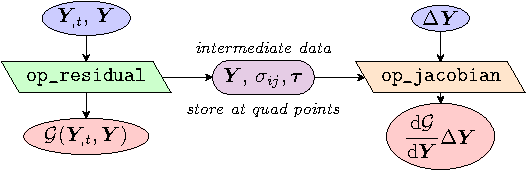
\includegraphics[width=1\textwidth]{img/op_jacobian.pdf}};

                    % Create scope with normalized axes
                    \begin{scope}[
                        x={($0.1*(image.south east)$)},
                        y={($0.1*(image.north west)$)}]

                        % % Grid
                        %     \draw[lightgray,step=1] (image.south west) grid (image.north east);
                        %
                        % % Axes' labels
                        %     \foreach \x in {0,1,...,10} { \node [below] at (\x,0) {\x}; }
                        %     \foreach \y in {0,1,...,10} { \node [left] at (0,\y) {\y};}

                        \invisible<3->{\draw[ultra thin,white,fill=white] (6.7, 0) rectangle (3.3, 10);}
                    \end{scope}
                \end{tikzpicture}
            \end{center}
        }
    \end{columns}
    \vspace{-20pt}
    \onslide<4->{
        \begin{itemize}
            \item \textbf{Pros:} Exact Jacobian matrix-vector product\footnote<5->{Affect of specific terms may be ignored from the Jacobian. This is done for \(\derd\bm{\tau}/\derd\bm{Y}\)}
            \item \textbf{Cons:} Preconditioning requires partial assembly, requires coding Jacobian
        \end{itemize}
    }
\end{frame}

% \begin{frame}{Performance Exact Matrix-Free Jacobian via CeedOperator}
%     \begin{columns}
%         \column{0.6\textwidth}
%         \onslide<+->{
%             \begin{figure}
%                 \centering
%                 \begin{tikzpicture}
%                     \node [
%                     above right,
%                     inner sep=0] (image) at (0,0) {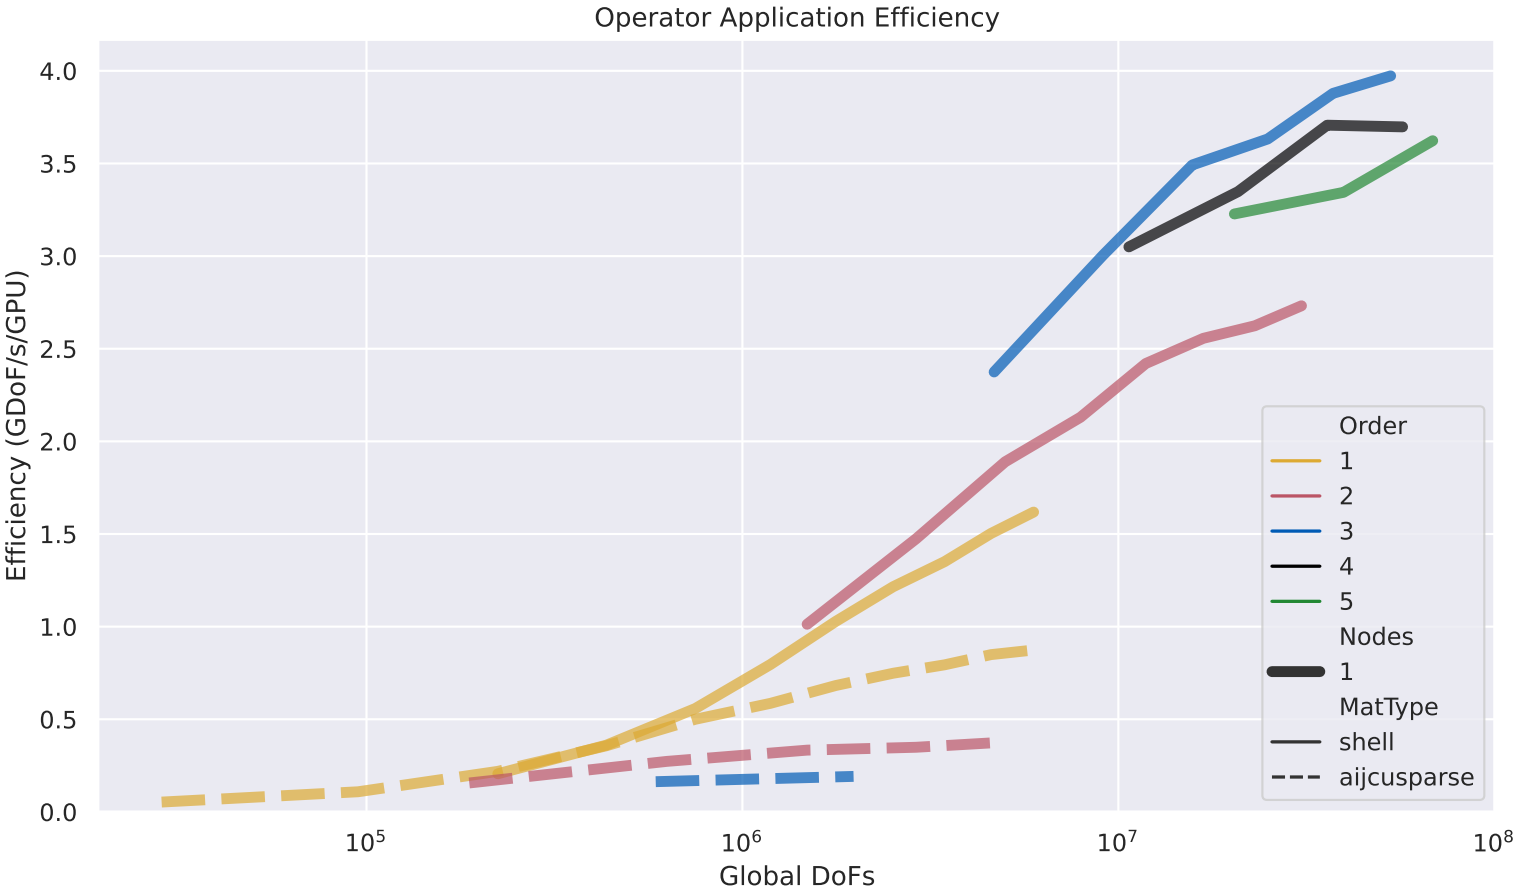
\includegraphics[width=1\textwidth]{img/OpAppEfficiency_PerfPortSolidsFig7.png}};
%
%                     % Create scope with normalized axes
%                     \begin{scope}[
%                         x={($0.1*(image.south east)$)},
%                         y={($0.1*(image.north west)$)}]
%
%                         % % Grid
%                         %     \draw[lightgray,step=1] (image.south west) grid (image.north east);
%                         %
%                         % % Axes' labels
%                         %     \foreach \x in {0,1,...,10} { \node [below] at (\x,0) {\tiny \x}; }
%                         %     \foreach \y in {0,1,...,10} { \node [left] at (0,\y) {\tiny \y};}
%
%                         % Performance is 0.66, 0.88, and 2.38 GDoFs/s/GPU for Q1,Q2, and Q3 respectively
%                         \onslide<+->{
%                             \draw[solids_yellow, fill=solids_yellow] (7.4, 2.32) circle(2pt);
%                             \draw[solids_red,    fill=solids_red]    (7.4, 2.76) circle(2pt);
%                             \draw[solids_blue,   fill=solids_blue]   (7.4, 5.76) circle(2pt);
%                         }
%                     \end{scope}
%                 \end{tikzpicture}
%                 \vspace{-10pt}
%                 \caption{\tiny Matrix-Free Application Comparison (Reproduced from Brown \textit{et al.} 2022). Not from fluids code, but representative of libCEED matrix-free}
%                 % Run on LLNL Lassen, 4xV100 GPUs. aijcusparse results in narrow DoFs range due to memory contraints.
%             \end{figure}
%         }
%
%         \column{0.45\textwidth}
%         \begin{itemize}
%                 \item<.-> Significant differences with performance implications
%                 \begin{itemize}
%                     \item<.-> Fluids run over 2 nodes \(\longrightarrow\) network latency present
%                     \item<.-> Solids code lower in FLOPs and storage per DoF
%                 \end{itemize}
%             \item<+-> Significant increase in efficiency for \(Q_1,\, Q_2 \rightarrow Q_3\)
%         \end{itemize}
%     \end{columns}
% \end{frame}

\section{Performance and Results of Flat Plate Boundary Layer Simulation}

\begin{frame}{Problem Description}
    \begin{itemize}
        \item Flat plate boundary layer with zero pressure gradient
            \begin{itemize}
                \item \(Re_\theta \approx 970\) boundary layer at inflow, \(M \approx 0.1\)
                \item Synthetic turbulence generation (STG) used for inflow structures
                \item Run at implicit large eddy simulation (ILES) resolution for linears (higher orders may be DNS level, tbd)
            \end{itemize}
        \item Test 3 different order elements, \(Q_1, Q_2, Q_3\) tensor-product hexes
        \item Maintain \textit{DOF resolution} (DoFs per physical length/ global DoF count)
        \item Performance results shown for two nodes of ALCF's Polaris (4\(\times\) NVIDIA A100 per node)
    \end{itemize}
\end{frame}

\begin{frame}{Exact Matrix-Free Jacobian vs Sparse}
    \begin{columns}
        \column{0.5\textwidth}
        \onslide<+->{
            \begin{figure}
                \centering
                \vspace{-5pt}
                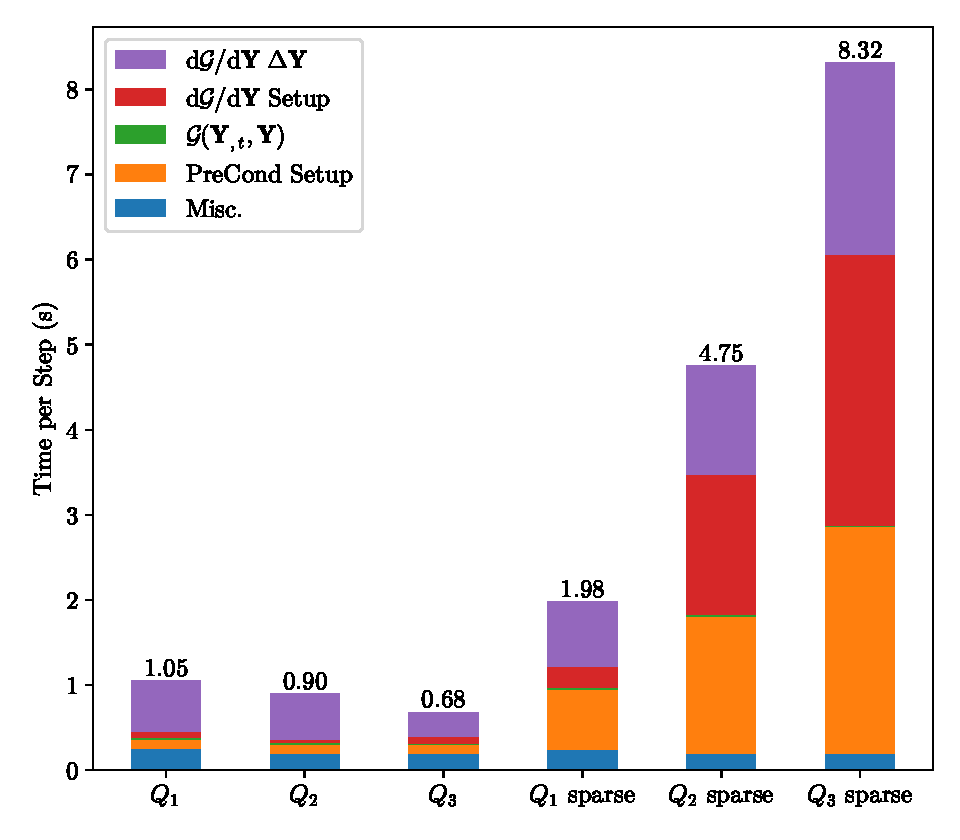
\includegraphics[width=1\textwidth]{img/PerformanceBarChart_sparse.pdf}
                \vspace{-30pt}
            \end{figure}
        }

        \column{0.5\textwidth}
        \begin{itemize}
            \item<+-> Sparse \(\derd \mathcal{G} / \derd \bm{Y} \Delta \bm{Y}\) significantly slower than matrix-free
            \item<+-> Time to assemble \(\derd \mathcal{G} / \derd \bm{Y}\) quite large
            \item<+-> Associated costs rise with element order
        \end{itemize}
    \end{columns}
\end{frame}

\begin{frame}{Fluids Performance Analysis}
    \begin{columns}
        \column{0.5\textwidth}
        \onslide<+->{
            \begin{figure}
                \centering
                \vspace{-5pt}
                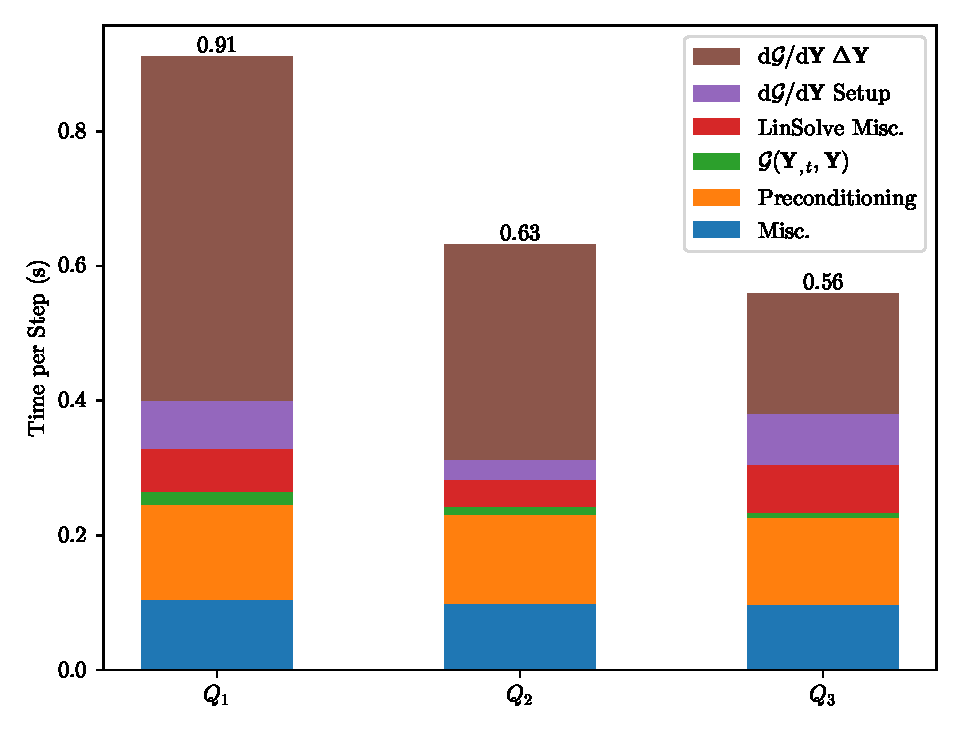
\includegraphics[width=1\textwidth]{img/PerformanceBarChart.pdf}
                \vspace{-30pt}
                % From looking at logs in /eagle/cfdml_aesp/PolarisMilestone/Cases/8part{,P2,P3}
                % Zulip discussion around here: https://phypid.zulipchat.com/#narrow/stream/232375-ceed-phasta/topic/field.20node.20blocking.20for.20P3.2B/near/321175758
            \end{figure}
        }

        \column{0.5\textwidth}
        \begin{itemize}
            \item<+-> Time of \(\derd \mathcal{G} / \derd \bm{Y} \Delta \bm{Y}\) decreases as order increases
            \item<+-> \(\derd \mathcal{G} / \derd \bm{Y}\) setup time increases with order
                \begin{itemize}[<.->]
                    \item Dominant cost is partial matrix assembly for preconditioning
                    % \item For \(Q_3\), eats up gains from faster \(\derd \mathcal{G} / \derd \bm{Y} \Delta \bm{Y}\) calculations
                \end{itemize}
        \end{itemize}
    \end{columns}
\end{frame}

\begin{frame}{Results of Flat Plate Boundary Layer}
    \begin{columns}
    \column{0.6\textwidth}
    \begin{figure}
        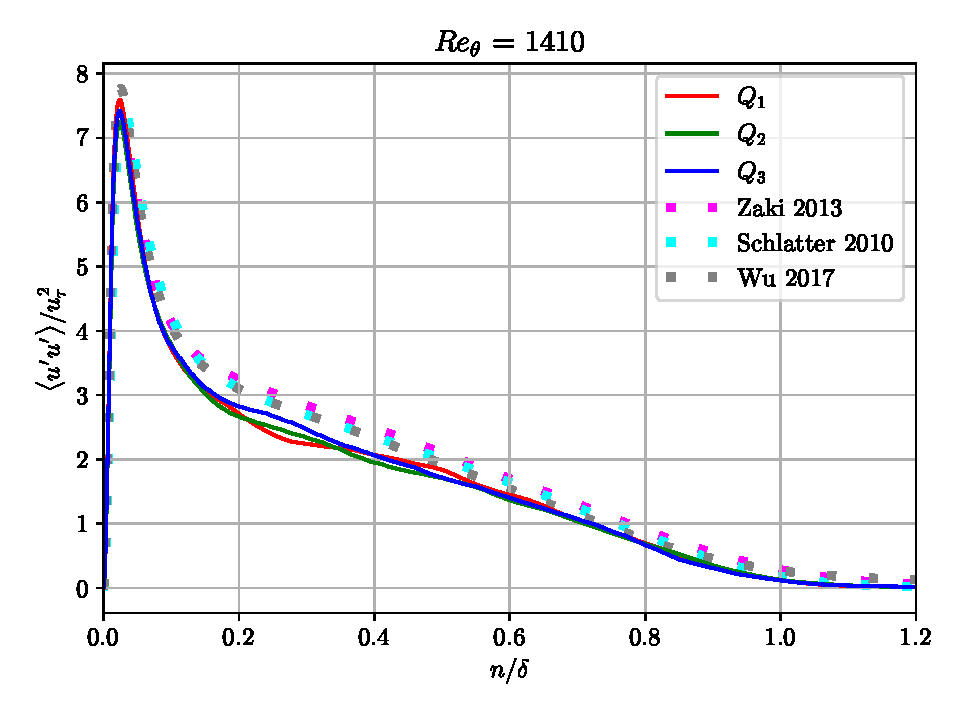
\includegraphics[width=1\textwidth]{img/upup_Re1410.pdf}
        \caption{asdf}
    \end{figure}

    \column{0.4\textwidth}
       \begin{itemize}
            \item Spanwise statistics implemented to verify scale-resolving results
            \item Results \textit{not} converged, but show realistic stress profiles
       \end{itemize}
       \tiny{Zaki \textit{et al.}, 2013, \textit{From Streaks to Spots and on to Turbulence: Exploring the Dynamics of Boundary Layer Transition}\\
       Schlatter \textit{et al.}, 2010, \textit{Assessment of direct numerical simulation data of turbulent boundary layers}\\
       Wu \textit{et al.}, 2017, \textit{Transitional–turbulent spots and turbulent–turbulent spots in boundary layers}\\}
    \end{columns}
\end{frame}

\begin{frame}{Support and References}
    \begin{itemize}
        \item Research supported by US Department of Energy through DE-SC0021411 FASTMath SciDAC Institute
        \item Argonne Leadership Computing Facility resources used for this research
        \item We thank PETSc and libCEED developers, especially Jeremy Thompson and Junchao Zhang among many others
    \end{itemize}
\end{frame}

\begin{frame}{Appendix Slides}

\end{frame}

\begin{frame}{Performance Exact Matrix-Free Jacobian via CeedOperator}
    \begin{columns}
        \column{0.6\textwidth}
        \onslide<+->{
            \begin{figure}
                \centering
                \begin{tikzpicture}
                    \node [
                    above right,
                    inner sep=0] (image) at (0,0) {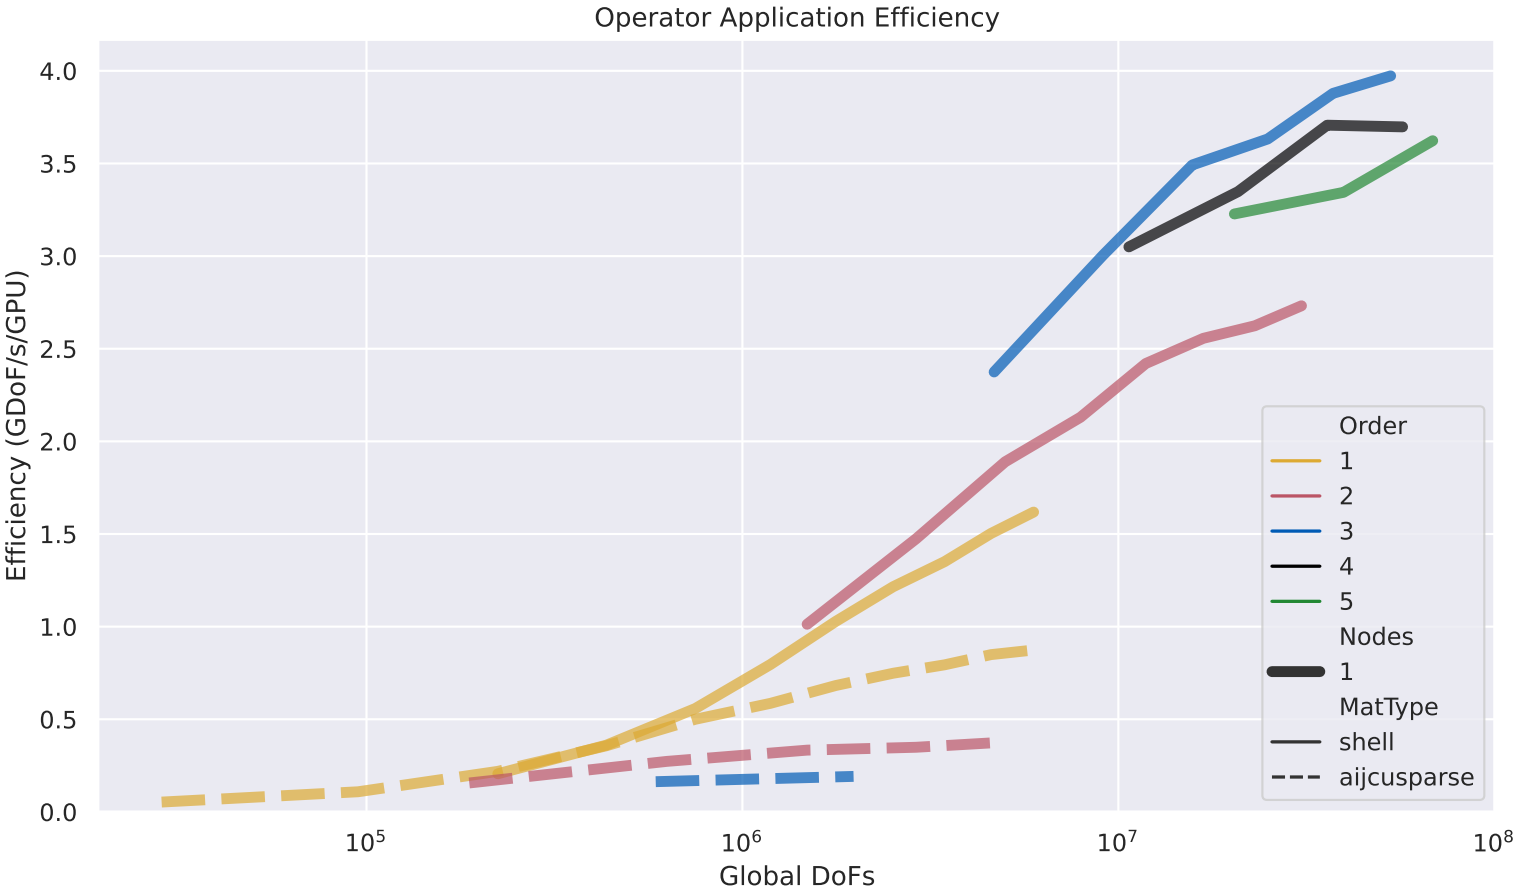
\includegraphics[width=1\textwidth]{img/OpAppEfficiency_PerfPortSolidsFig7.png}};

                    % Create scope with normalized axes
                    \begin{scope}[
                        x={($0.1*(image.south east)$)},
                        y={($0.1*(image.north west)$)}]

                        % % Grid
                        %     \draw[lightgray,step=1] (image.south west) grid (image.north east);
                        %
                        % % Axes' labels
                        %     \foreach \x in {0,1,...,10} { \node [below] at (\x,0) {\tiny \x}; }
                        %     \foreach \y in {0,1,...,10} { \node [left] at (0,\y) {\tiny \y};}

                        % Performance is 0.66, 0.88, and 2.38 GDoFs/s/GPU for Q1,Q2, and Q3 respectively
                        \onslide<+->{
                            \draw[solids_yellow, fill=solids_yellow] (7.4, 2.32) circle(2pt);
                            \draw[solids_red,    fill=solids_red]    (7.4, 2.76) circle(2pt);
                            \draw[solids_blue,   fill=solids_blue]   (7.4, 5.76) circle(2pt);
                        }
                    \end{scope}
                \end{tikzpicture}
                \vspace{-10pt}
                \caption{\tiny Matrix-Free Application Comparison (Reproduced from Brown \textit{et al.} 2022). Not from fluids code, but representative of libCEED matrix-free}
                % Run on LLNL Lassen, 4xV100 GPUs. aijcusparse results in narrow DoFs range due to memory contraints.
            \end{figure}
        }

        \column{0.45\textwidth}
        \begin{itemize}
                \item<.-> Significant differences with performance implications
                \begin{itemize}
                    \item<.-> Fluids run over 2 nodes \(\longrightarrow\) network latency present
                    \item<.-> Solids code lower in FLOPs and storage per DoF
                \end{itemize}
            \item<+-> Significant increase in efficiency for \(Q_1,\, Q_2 \rightarrow Q_3\)
        \end{itemize}
    \end{columns}
\end{frame}

\end{document}

% \begin{frame}{Flat Plate Boundary Layer, Zero Pressure Gradient}
%     Problem Description:
%     \begin{itemize}
%         \item \(Re_\theta \approx 970\) boundary layer at inflow, \(M \approx 0.1\)
%         \item Synthetic turbulence generation (STG) used for inflow structures
%         \item Internal damping layer (IDL) used in STG development region to prevent pressure wave growth
%         \item \textcolor{red}{asdf}
%         \item Domain size of \(\{27 \times 24 \times 4\} \delta_0\)
%     \end{itemize}
% \end{frame}

% \begin{frame}{High-Order Approach}
%     \begin{itemize}
%         \item Test 3 different order elements, \(Q_1, Q_2, Q_3\) tensor-product hexes
%         \item Maintain \textit{DOF resolution} (DOFs per physical length)
%         \item DOF resolution for streamwise and spanwise was \(\Delta x^+ = 30\) and \(\Delta z^+ = 12\)
%             \begin{itemize}
%                 \item For \(Q_1\), this is about half the resolution required for DNS resolution
%             \end{itemize}
%     \end{itemize}
% \end{frame}

% \section{A (Very) Brief Finite Element Refresher}
%
% \begin{frame}{Galerkin Form}
%
%         \onslide<+-> {Given the homogenous Poisson equation in weak form: Find \(u \in \mathcal{S}\) such that
%             \begin{equation*}
%                 \int_\Omega v_{,x} u_{,x} \dif \Omega = \int_\Omega vf \dif \Omega \quad \forall v \in \mathcal{V}
%             \end{equation*}}
%
%         \onslide<+-> {
%             Approximate \(\mathcal{S} \approx \mathcal{S}^h = \Span(\{\phi^i\}_i^\ndof)\) and \(\mathcal{V} \approx \mathcal{V}^h = \Span(\{\phi^j\}_j^\ndof)\)
%         }
%         \onslide<+->{
%             \begin{equation*}
%                 \bm{Ax} = \bm{b}
%             \end{equation*}
%         }
%         \onslide<+->{
%             \begin{equation*}
%                 u = \sum_i^\ndof \phi^i x_i \in \mathcal{S}^h, \quad A_{ij} = \int_{\Omega} \phi^i_{,x} \phi^j_{,x} \dif \Omega, \quad b_j = \int_\Omega \phi^j f \dif \Omega
%             \end{equation*}
%         }
%
% \end{frame}

% \begin{frame}{Finite Element Method}
%         \onslide<+-> {
%             Discretize the domain \(\Omega\) into elements \(\Omega^e\)
%             \begin{equation*}
%                 \Omega^h = \bigcup_{e=0}^{\nelm} \Omega^e \approx \Omega
%             \end{equation*}
%         }
%         % \onslide<+-> {
%         %     Define finite element function spaces:
%         %     \begin{equation*}
%         %         \mathcal{S}^h \coloneqq \left\{ v^h \in \mathcal{F}(\Omega^h)\right\}
%         %     \end{equation*}
%         % }
%         % \onslide<+-> {
%         %     \begin{equation*}
%         %         A_{ij} = \sum_e^\nelm \int_{\Omega^e} \phi^i_{,x} \phi^j_{,x} \dif \Omega, \quad b_j = \sum_e^\nelm \int_{\Omega^e} \phi^j f \dif \Omega
%         %     \end{equation*}
%         % }
%         \onslide<+->{
%             Approximate the integrals over elements via quadrature \[\int g(x) \dif x \approx \sum_k^\nquad w^k g(\xi^k)\]
%         }
%         \onslide<+->{
%             Thus the final problem can be stated as: Find \(\bm{x} \in \mathbb{R}^\ndof\) in \(\bm{Ax} = \bm{b}\) for
%             \begin{equation*}
%                 A_{ij} = \sum_e^\nelm \sum_k^\nquad \left[ w^k \phi^i_{,x}(\xi^k) \phi^j_{,x}(\xi^k) \right]_{\Omega^e}, \quad b_j = \sum_e^\nelm \sum_k^\nquad \left[ w^k \phi^j(\xi^k) f(\xi^k) \right]_{\Omega^e}
%             \end{equation*}
%         }
%
% \end{frame}


% ------------ Backup slides (old ones that may get reused later)
% \begin{frame}{libCEED Operator}
%
%     \begin{columns}
%         \column{0.4\textwidth}
%         \begin{center}
%             \begin{tabular}{ c c c }
%             Operator & libCEED Object\\ [0.5ex]
%             \hline\hline
%             \onslide<+->{\(\Elem\)   & \footnotesize\texttt{CeedElemRestriction} \\}
%             \onslide<+->{\(\Bas\)    & \footnotesize\texttt{CeedBasis} \\}
%             \onslide<+->{\(\DQfunc\) & \footnotesize\texttt{CeedQFunction} \\}
%             \onslide<+->{\(\ElemT\BasT\DQfunc\Bas\Elem\) & \footnotesize\texttt{CeedOperator}}
%             \end{tabular}
%         \end{center}
%
%         \column{0.6\textwidth}
%             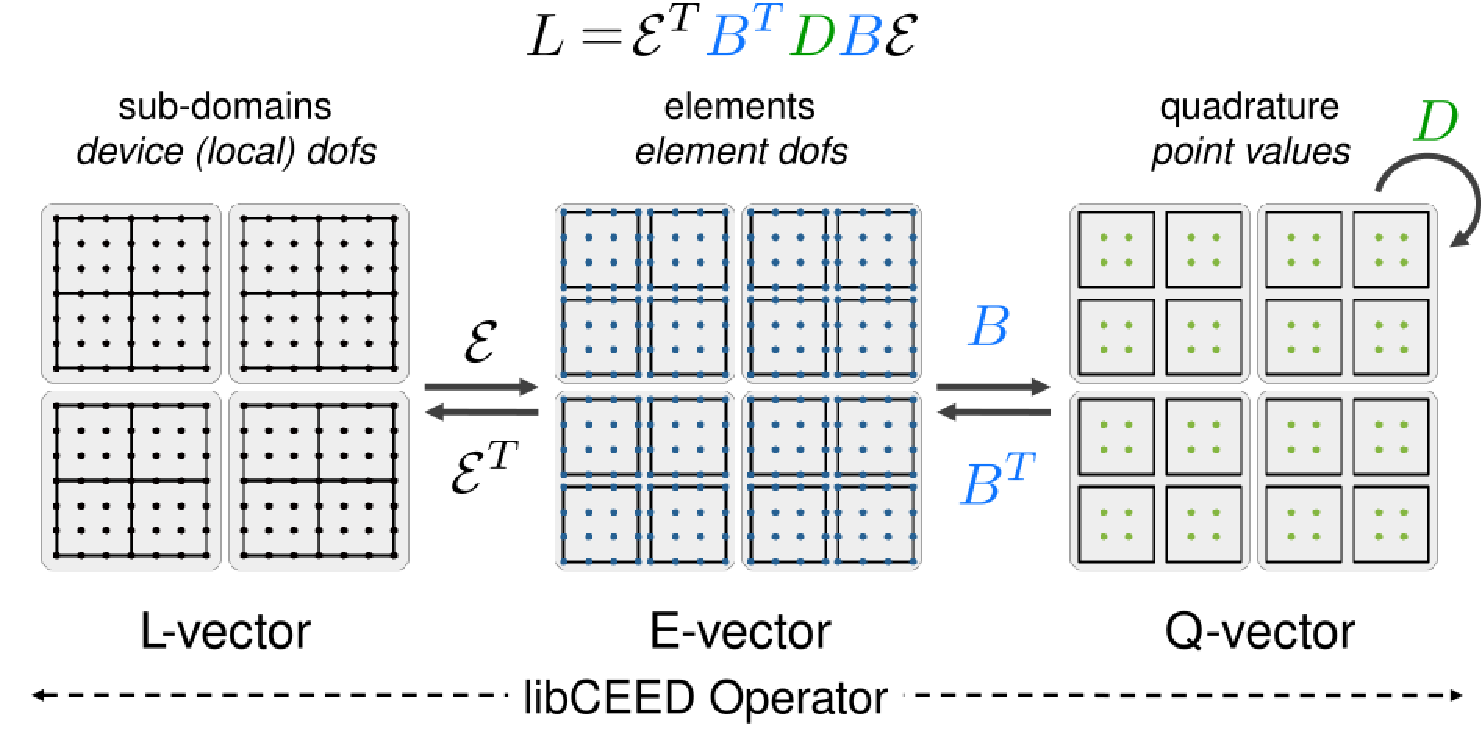
\includegraphics[width=\textwidth]{img/libCEED_Operator.pdf}
%     \end{columns}
%     \begin{block}{Note}<+->
%         libCEED implements the operators matrix-free; None of the libCEED Objects store a matrix
%     \end{block}
% \end{frame}

% \begin{frame}{Defining the libCEED Operator}
%
%     \begin{columns}
%         \column{0.5\textwidth}
%         \onslide<1->{
%             \footnotesize\texttt{CeedElemRestriction}
%             \begin{itemize}
%                 \item Defined by element connectivity and the number of components
%             \end{itemize}
%         }
%         \onslide<2->{
%             \footnotesize\texttt{CeedBasis}
%             \begin{itemize}
%                 \item Defined by the basis functions and the quadrature rule
%                 \item Built-in options for common basis functions and quadrature rules
%             \end{itemize}
%         }
%
%         \column{0.5\textwidth}
%         \onslide<3->{
%             \footnotesize\texttt{CeedQFunction}
%             \begin{itemize}
%                 \item C function
%                 \item Common operators available (mass, poisson, identity, etc.)
%                 \item User defined QFunctions also possible
%             \end{itemize}
%         }
%
%         \onslide<4->{
%             \footnotesize\texttt{CeedOperator}
%             \begin{itemize}
%                 \item Computation backend defined at runtime
%                 \item Full \(L\) operator (can be) JITed to the desired backend (CUDA, HIP, CPU, etc.)
%             \end{itemize}
%         }
%     \end{columns}
% \end{frame}

% \begin{frame}[fragile]{Poisson CeedQFunction}
%     \begin{columns}
%
%         \column{0.4\textwidth}
%         \onslide<1->{
%             \[ \sum_k^\nquad \left[ w^k u_{,x}(\xi^k) v_{,x}(\xi^k) \right]_{\Omega^e} \]
%             \vspace{-20pt}
%             \[\BasT\DQfunc\Bas\]
%         }
%         \vspace{-20pt}
%         \begin{itemize}
%             \item<2-> \texttt{ug=} \(u_{,x}(\xi^k) = \Bas u^e\)
%             \item<3-> \texttt{q\char`_data=} \(w^k\)\footnote<3->{along with jacobian determinant}
%             \item<4-> \texttt{vg=} \(w^k u_{,x}(\xi^k) = \DQfunc\Bas u^e\)
%             \item<5-> \(w^k u_{,x}(\xi^k) v_{,x}(\xi^k) = \BasT \DQfunc \Bas u^e\)
%         \end{itemize}
%
%     \column{0.6\textwidth}
% % \onslide<2->{
% \begin{ccode}
% CEED_QFUNCTION(Poisson1DApply)(void *ctx, const CeedInt Q,
%                                const CeedScalar *const *in,
%                                CeedScalar *const *out) {
%   // in[0] is gradient u, size (Q)
%   // in[1] is quadrature data, size (Q)
%   const CeedScalar *ug = in[0], *q_data = in[1];
%
%   // out[0] is output to multiply against gradient v, size (Q)
%   CeedScalar *vg = out[0];
%
%   // Quadrature point loop
%   CeedPragmaSIMD
%   for (CeedInt i=0; i<Q; i++) {
%     vg[i] = ug[i] * q_data[i];
%   } // End of Quadrature Point Loop
%
%   return CEED_ERROR_SUCCESS;
% }
% \end{ccode}
% % }
%
%     \end{columns}
% \end{frame}

% ---- Conservative Variable Formulation Slides: ---

% \begin{frame}{Compressible Navier-Stokes}
%
%
%     \begin{equation*}
%         \bm{U}_{,t} + \bm{F}_{i,i}(\bm{U}) - S(\bm{U}) = 0
%     \end{equation*}
%
%     for
%
%     \begin{equation*}
%         \bm{U} =
%         \begin{bmatrix}
%             \rho \\
%             \rho u_i\\
%             E \equiv \rho e
%         \end{bmatrix}, \quad
%     \bm{F}_i(\bm{U}) =
%     \underbrace{
%         \begin{pmatrix}
%             \rho u_i\\
%             \rho u_i u_j + p \delta_{ij} \\
%             (\rho e + p)u_i
%         \end{pmatrix}}_{\bm F_i^{\text{adv}}} +
%     \underbrace{
%         \begin{pmatrix}
%         0 \\
%         -  \sigma_{ij} \\
%         - \rho u_j  \sigma_{ij} - k T_{,i}
%         \end{pmatrix}}_{\bm F_i^{\text{diff}}}, \quad
%     S(\bm{U}) =
%     - \begin{pmatrix}
%         0\\
%         \rho \bm{g} \\
%         0
%     \end{pmatrix}
%     \end{equation*}
%
%     \todo{convert to primitive variable formulation}
% \end{frame}
%
% \begin{frame}{Compressible Navier-Stokes for FEM}
%
%     Find \(\bm{U}\in \mathcal{S}^h\)
%     \begin{equation*}
%         \begin{aligned}
%             \int_{\Omega} \bm v \cdot \left( \bm{U}_{,t} - \bm{S}(\bm{U}) \right)  \,\dif \Omega
%             - \int_{\Omega} \bm{v}_{,i} \cdot \bm{F}_i(\bm{U})\, \dif\Omega & \\
%             + \int_{\partial \Omega} \bm v \cdot \bm{F}_i(\bm{U}) \cdot \widehat{\bm{n}}_i \,\dif \partial \Omega & \\
%             \onslide<2->{\underbrace{+ \int_{\Omega} \mathcal{P}(\bm v)^T \, \left(\bm{U}_{,t} + \bm{F}_{i,i}(\bm{U}) - S(\bm{U})
%              \right) \,\dif \Omega}_{\textrm{SUPG}} &= 0 \, , \; \forall \bm v \in \mathcal{V}^h \,}
%         \end{aligned}
%     \end{equation*}
%
%     \onslide<3->{
%         Further simplified into residual form:
%         \begin{align*}
%             \mathcal{G}(\bm{U}_{,t}, \bm{U}) &=0 \\
%             \onslide<4->{\Rightarrow \quad \PartT \ElemT \BasT \Qfunc{G} \Bas \Elem \Part &= 0}
%         \end{align*}
%     }
% \end{frame}

% ---- END Conservative Variable Formulation Slides: ---
